\documentclass[border=2mm]{standalone}
\usepackage[utf8]{inputenc}
\usepackage[english]{babel}
\usepackage{tikz}
% \usepackage[margin=1cm]{geometry}
\usepackage[most]{tcolorbox}
\usepackage{bm}
\usetikzlibrary{automata,positioning}

\begin{document}
    \begin{tcolorbox}[
        colback=white, % Couleur de fond de la boîte
        colbacktitle=white, % Couleur de fond du titre de la boîte
        coltitle=black, % Couleur du titre de la boîte
        colframe=black, % Couleur du cadre de la boîte
        arc=2mm, % Rayon de l'arrondi des coins
        boxrule=2pt, % Épaisseur du cadre de la boîte
        % breakable, enhanced jigsaw,
        width=15cm,
        height=4.8cm,
        title=\LARGE \textbf{ONLINE :} Apply enriched FEM,
        halign title=center
        ]

        \centering
        \begin{tikzpicture}
%            \draw[draw=black,dashed] (0,0) rectangle ++ (5.5,2.5);
%            \node at (2.75,1.85) {\Large \textbf{Inputs}};
%            \node[anchor=west] at (0.1,1.1) {\large $\bm{x}\in\Omega$ : spatial coordinates};
%            \node[anchor=west] at (0.1,0.5) {\large $\bm{\mu}\in\mathcal{M}$ : 1 given parameter};
            \node[draw=black,dashed,align=center,yshift=-2em] at (0.0,1.85) {
             \Large \textbf{Inputs} \\[0.50em]
             \large $\bm{x}\in\Omega$: spatial coordinates \\[.40em]
             \large \large $\bm{\mu}\in\mathcal{M}$: 1 given parameter\\[.10em]
            };

%            \draw[->, black, line width=2pt] (6,1.25) -- (7,1.25);
%            \node[draw=none, inner sep=0pt] at (9,1.55) {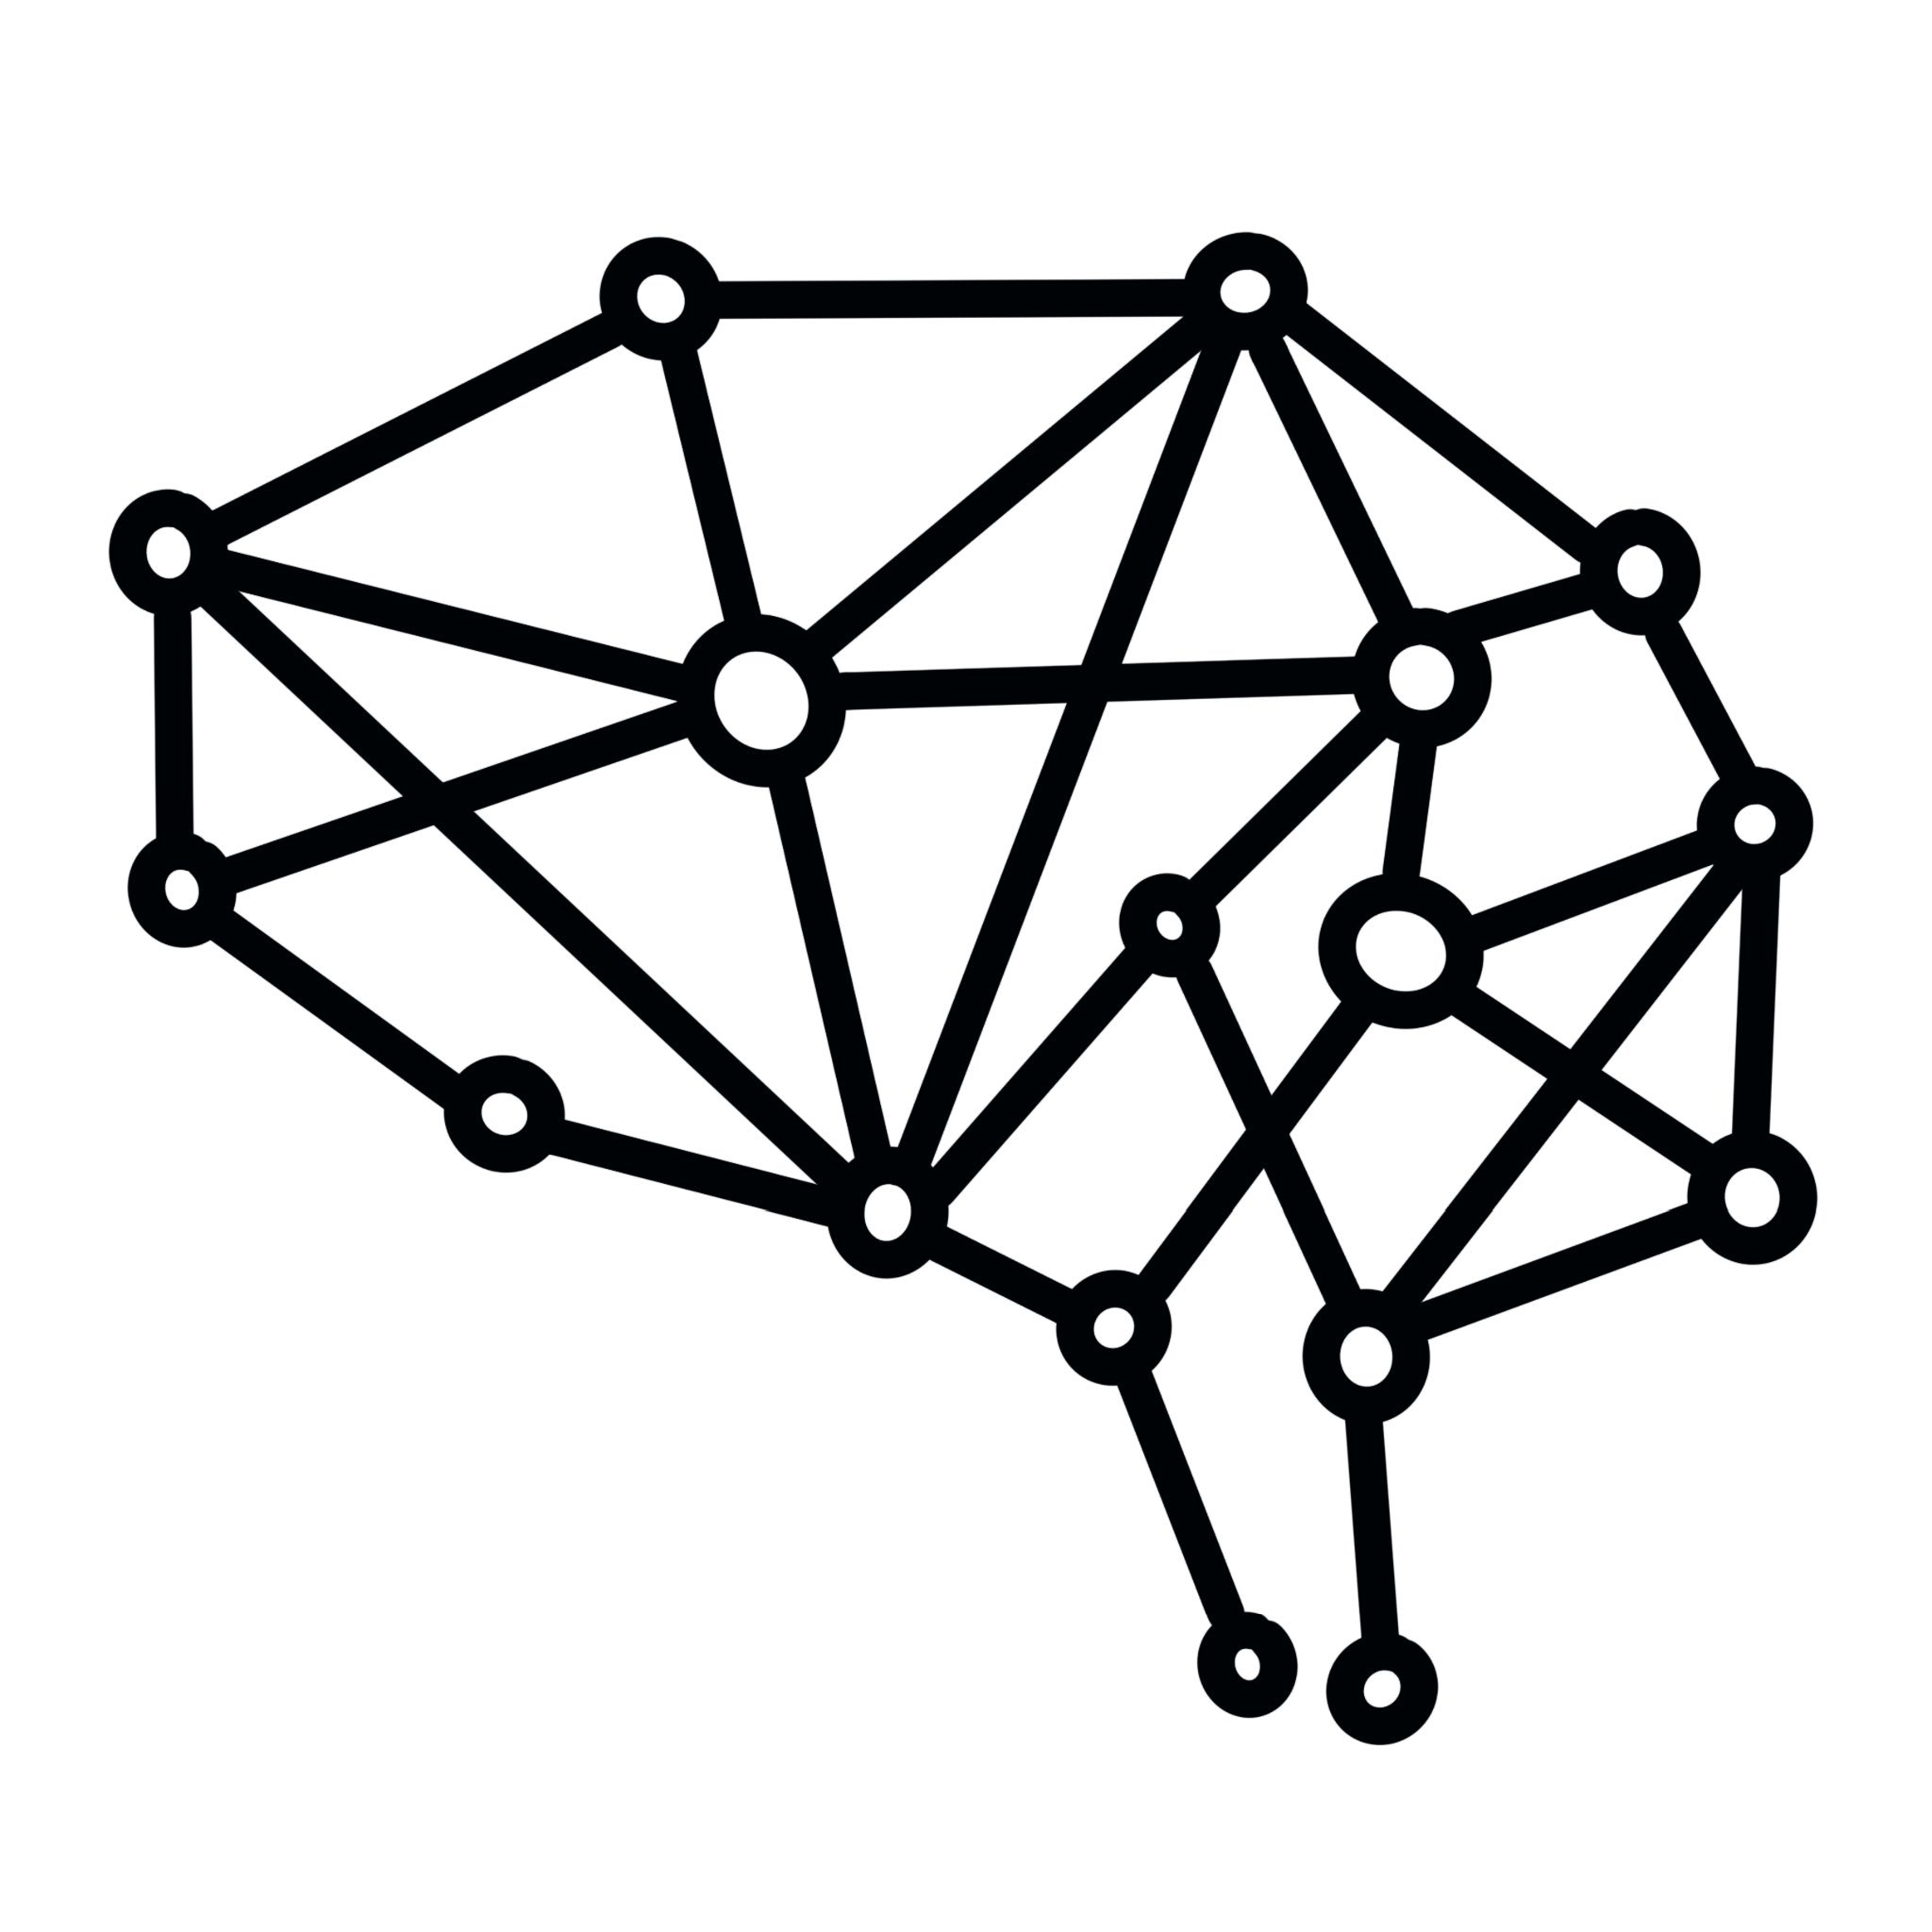
\includegraphics[width=2cm]{brain.pdf}};
%            \node at (9,0.35) {\large \textbf{Get PINN prediction}};
%            \draw[->, black, line width=2pt] (11,1.25) -- (12,1.25);

            \draw[->, black, line width=2pt] (2.9,1.25) -- (4.0,1.25);
            \node at (5.00,0.35) {\large \textbf{Get PINN prediction}};
            \node[draw=none, inner sep=0pt] at (4.8,1.55) {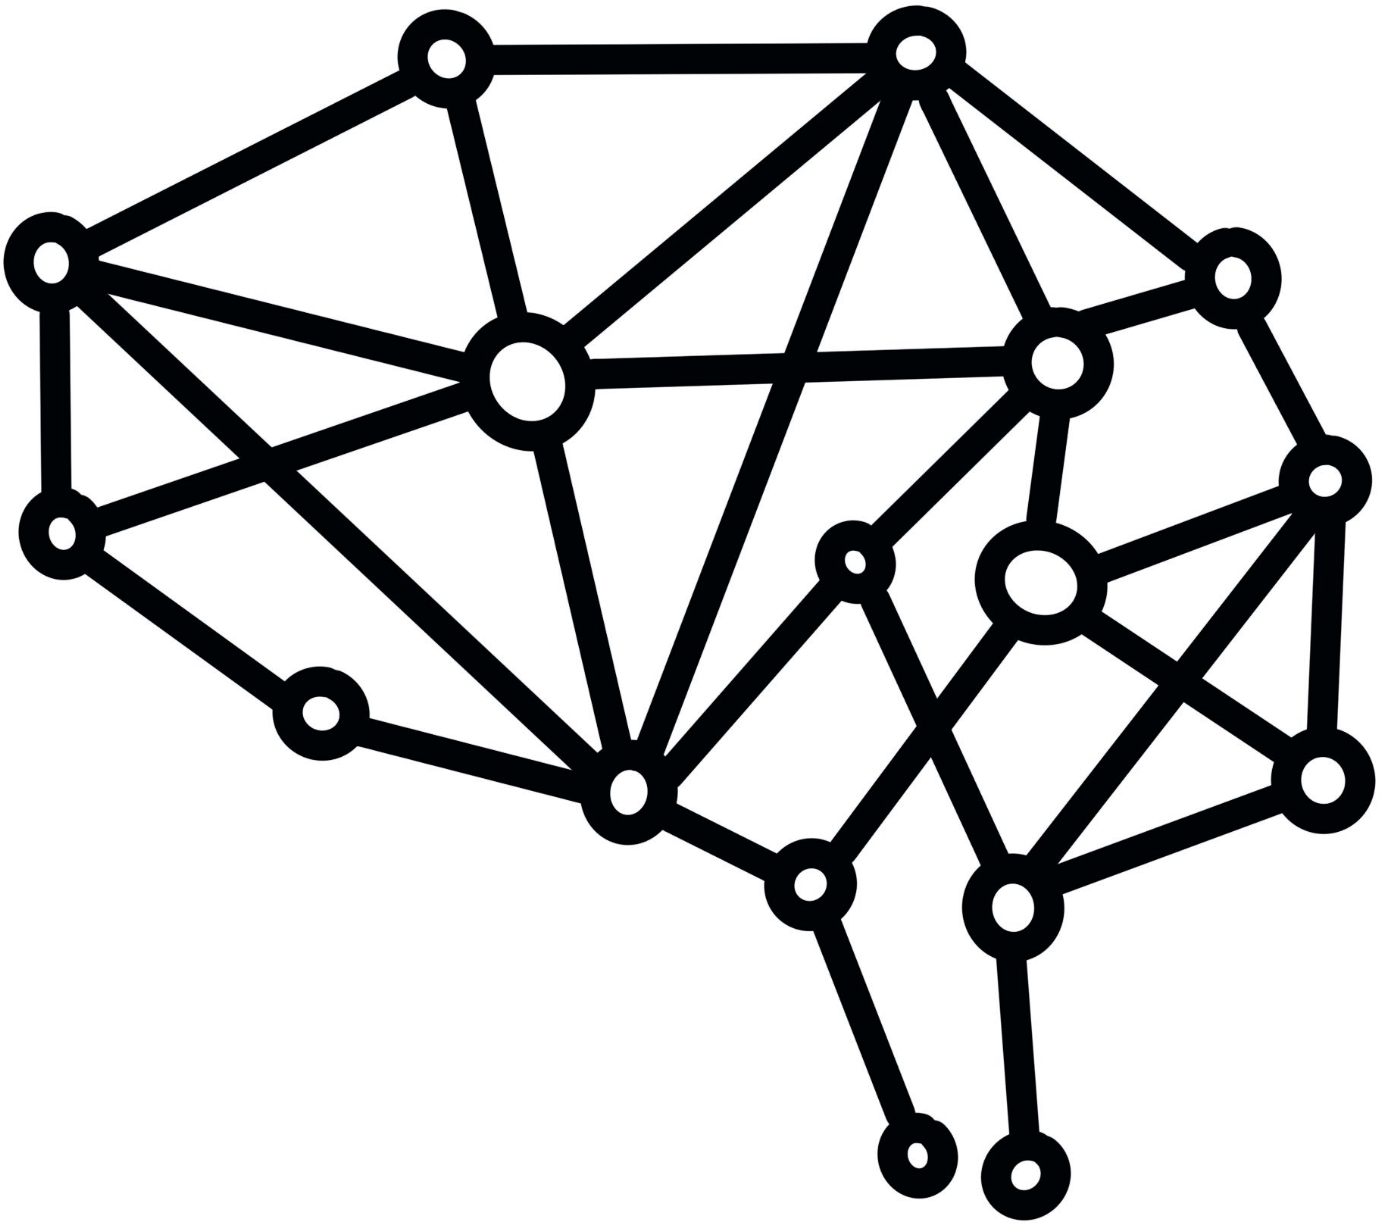
\includegraphics[width=2cm]{brain.png}};
            \draw[->, black, line width=2pt] (6,1.25) -- (7.1,1.25);

%            \draw[draw=black,dashed] (12.5,-0.25) rectangle ++ (5.5,3);
%            \node at (15.25,2.35) {\large \textbf{Correct PINN prediction}};
%            \node[draw=none, inner sep=0pt] at (15.25,1) {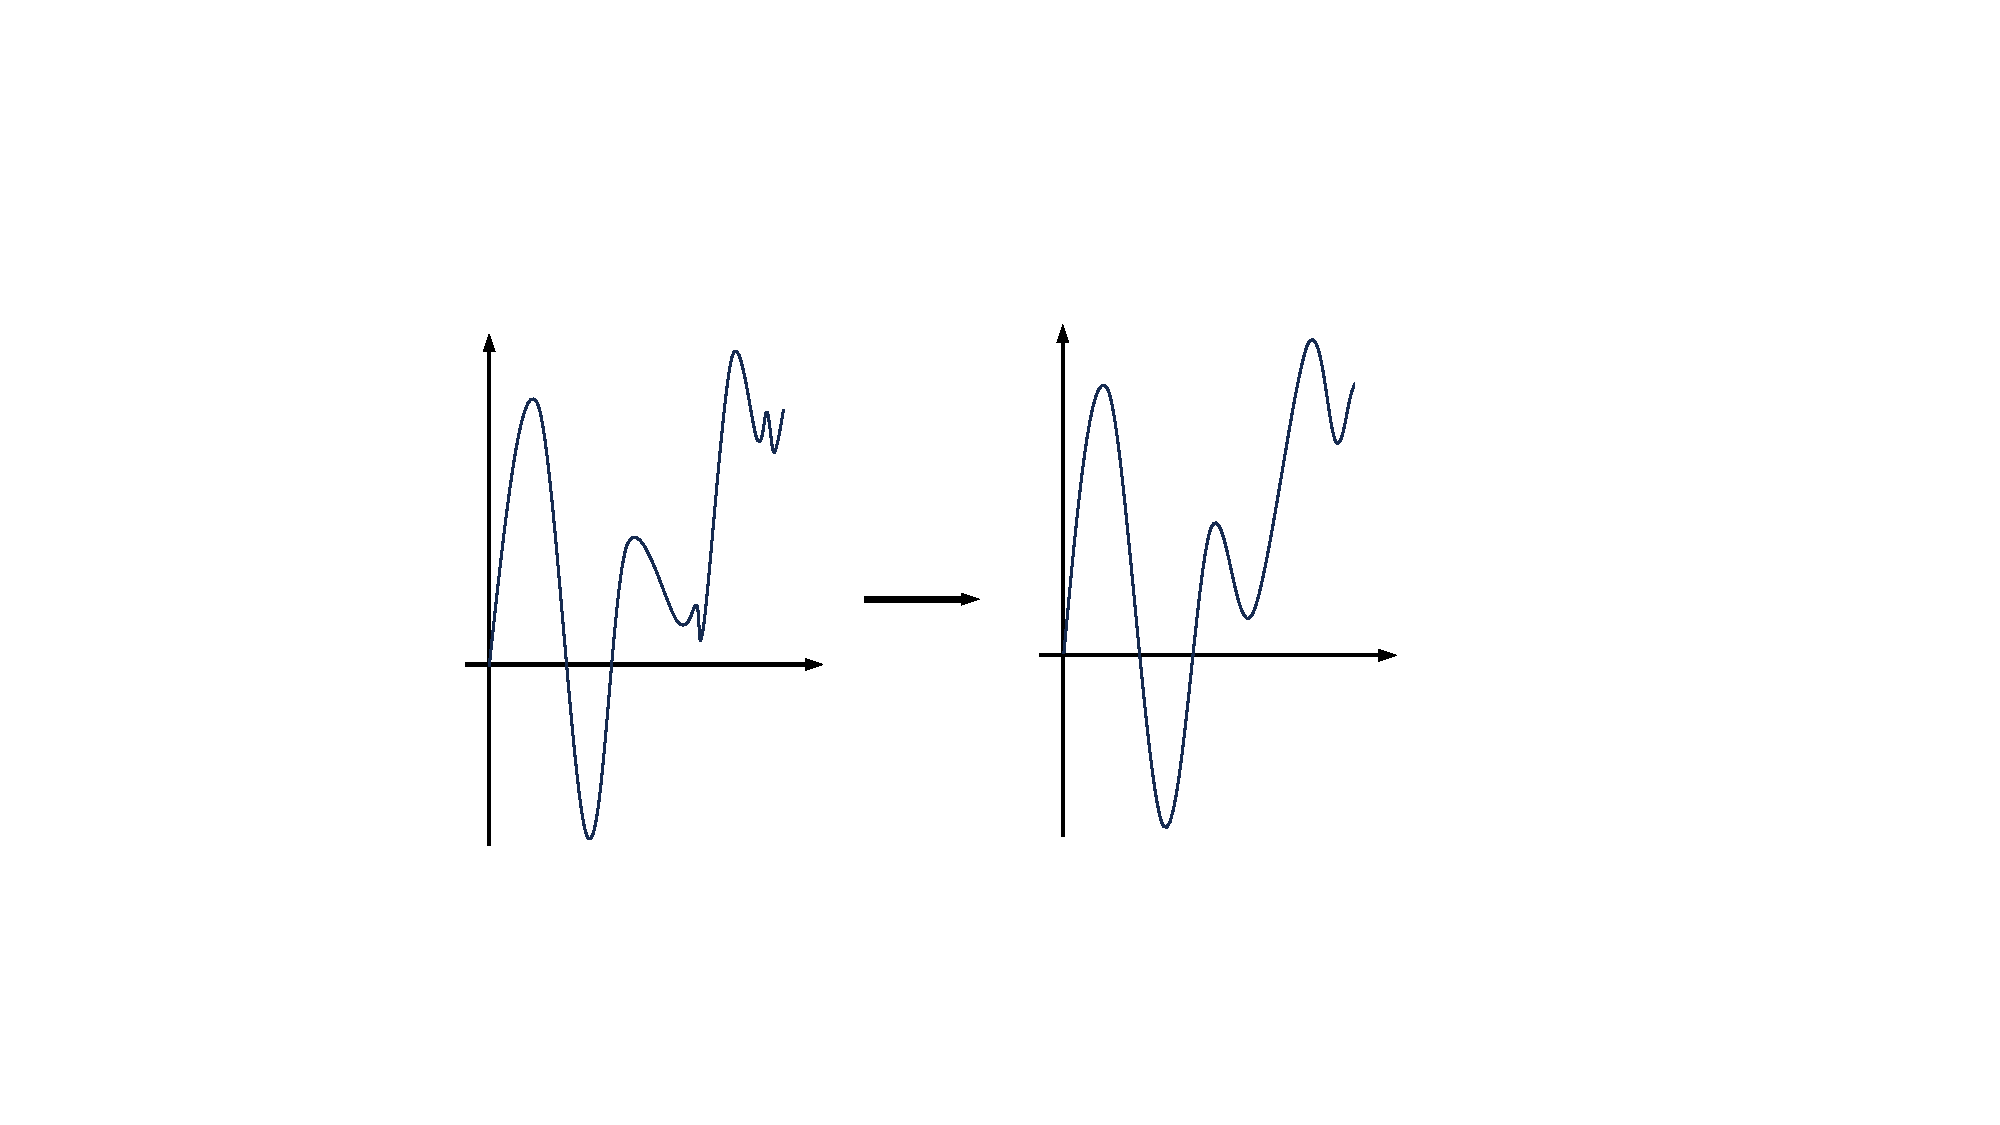
\includegraphics[width=4cm]{correction.pdf}};

            \node[draw=black,dashed,align=center,yshift=-2em,text width=11.5em] at (9.5,1.85) {
            \Large \textbf{Correct PINN prediction}: \\[.00em]
            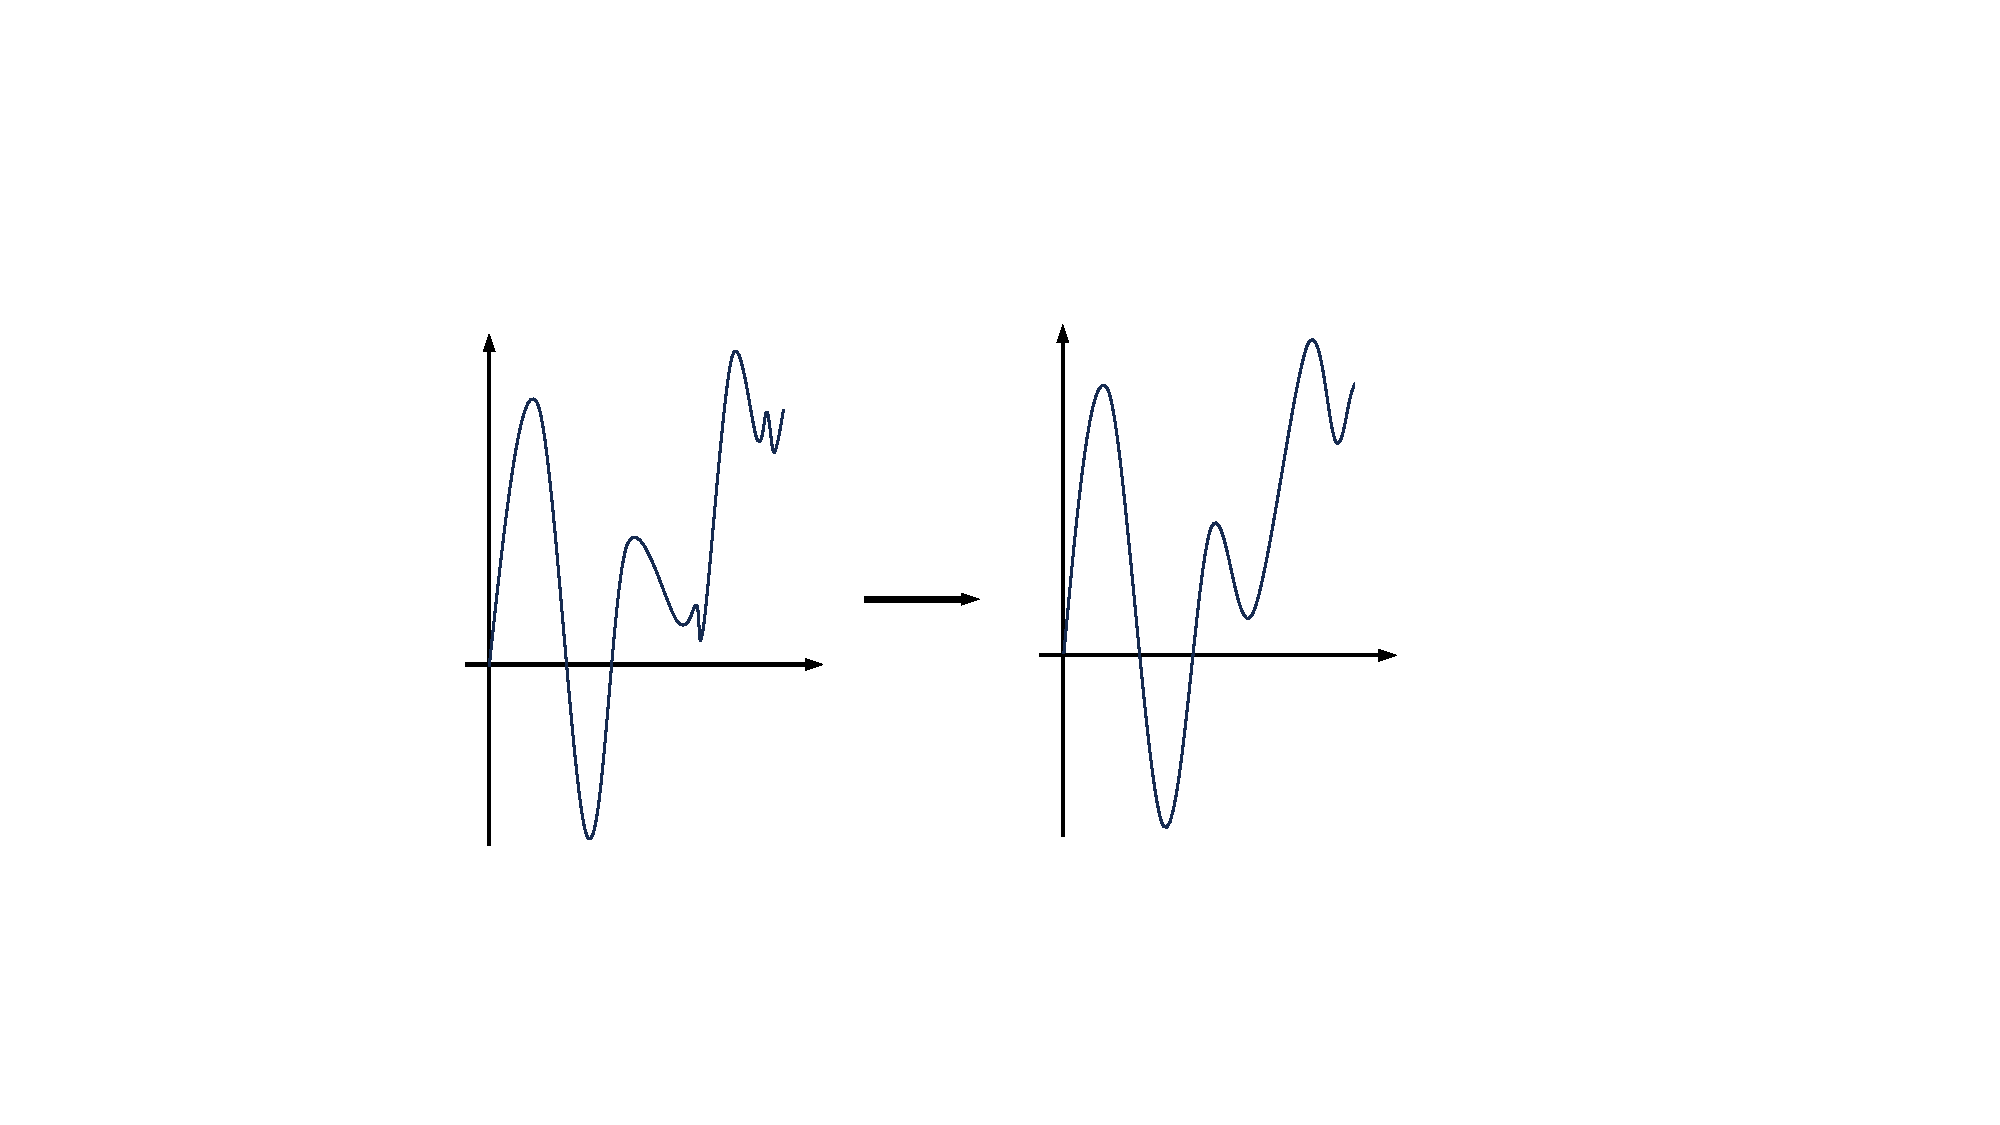
\includegraphics[width=4cm,height=3.5em]{correction.pdf}
            };


        \end{tikzpicture}
    \end{tcolorbox}
\end{document}
